\documentclass[UTF8, 12pt, a4paper, oneside]{ctexart}
\usepackage{listing}

\usepackage{amsmath}
\usepackage{amsfonts}
\usepackage{geometry}
\usepackage{ulem}
\usepackage[most]{tcolorbox}
\usepackage[hidelinks]{hyperref}
\usepackage{color}
\usepackage{framed}
\usepackage{mathtools,amssymb}
\usepackage{bm}

\lstset{
    basicstyle          =   \sffamily,          % 基本代码风格
    keywordstyle        =   \bfseries,          % 关键字风格
    commentstyle        =   \rmfamily\itshape,  % 注释的风格,斜体
    stringstyle         =   \ttfamily,  % 字符串风格
    flexiblecolumns,                % 别问为什么,加上这个
    numbers             =   left,   % 行号的位置在左边
    showspaces          =   false,  % 是否显示空格,显示了有点乱,所以不现实了
    numberstyle         =   \zihao{-5}\ttfamily,    % 行号的样式,小五号,tt等宽字体
    showstringspaces    =   false,
    captionpos          =   t,      % 这段代码的名字所呈现的位置,t指的是top上面
    frame               =   lrtb,   % 显示边框
}

\lstdefinestyle{C++}{
    language        =   C++, % 语言选Python
    basicstyle      =   \zihao{-5}\ttfamily,
    numberstyle     =   \zihao{-5}\ttfamily,
    keywordstyle    =   \color{blue},
    keywordstyle    =   [2] \color{teal},
    stringstyle     =   \color{magenta},
    commentstyle    =   \color{red}\ttfamily,
    breaklines      =   true,   % 自动换行,建议不要写太长的行
    columns         =   fixed,  % 如果不加这一句,字间距就不固定,很丑,必须加
    basewidth       =   0.5em,
}

\title{CSP 202203 实验报告}
\author{学号:2022212408 姓名:胡宇杭}
\date{\today}

\begin{document}
\maketitle
\section*{提交结果}
\begin{figure*}[htbp]
    \centering
    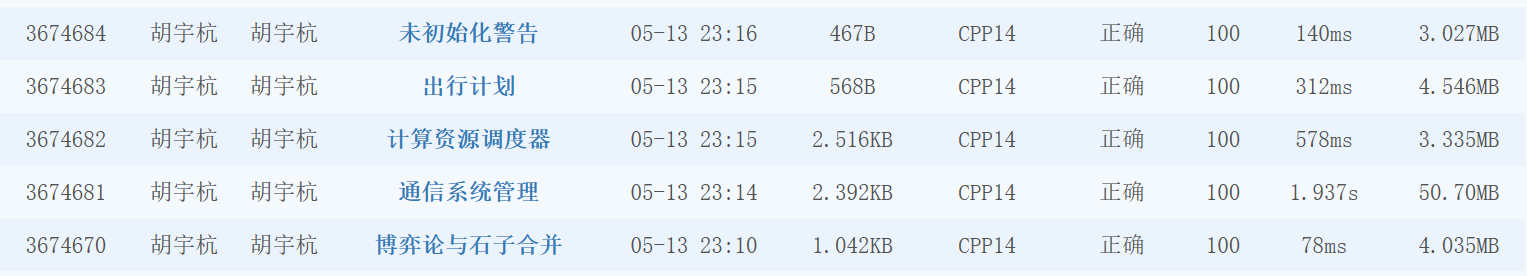
\includegraphics[width = 5in]{提交结果.png}
    \caption{提交结果}
\end{figure*}
\section{202203-1 未初始化警告}
\begin{itemize}
    \item 时间限制: $1.0\texttt{ s}$
    \item 空间限制: $512.0\texttt{ MB}$
\end{itemize}
\subsection{题目}
\subsubsection{问题描述}
\par 考虑一段包含 $k$ 条赋值语句的简单代码。 该段代码最多使用到 $n$ 个变量,分别记作 $a_1, a_2, \cdots, a_n$;常量用$a_0$表示。
\par 对于任意一条赋值语句 $a_{x_i} = a_{y_i}$,如果右值 $a_{y_i}$ 是一个变量,则其应该在此之前被初始化过,否则认为该条语句存在右值未初始化的问题。
\par 按照上述规则,试统计给定的代码中,有多少条赋值语句右值未被初始化。
\subsubsection{子任务}
\par $50\%$ 的测试数据满足 $0 < n,k\leq 1000$;
\par 全部的测试数据满足 $0 < n,k\leq 10^5$。
\subsection{题解}
\subsubsection{解法一 (100分)}
\par 在一条赋值语句中,无论右值是否被初始化过,左值都会被初始化,因此可以定义 $initial$ 数组,对于每一个变量 $i$,$initial[i]$记录该变量是否被初始化过。初始时将$initial[0]$赋值为真,表示常数。
\begin{itemize}
    \item 时间复杂度: $O(k)$
    \item 空间复杂度: $O(n)$
\end{itemize}
\subsubsection{C++代码实现}
\lstinputlisting[
    style = C++,
    title = {\bf 202203-1 未初始化警告}
]{test01.cpp}


\section{202203-2 出行计划}
\begin{itemize}
    \item 时间限制:$1.5\texttt{ s}$
    \item 空间限制:$512.0\texttt{ MB}$
\end{itemize}
\subsection{题目}
\subsubsection{问题描述}
\par 在某个神奇的地方,出入各个场所都要持有一定时间内的核酸检测阴性证明。若在 $t$ 时刻做了核酸,在等待 $k$ 时间后可以获得核酸证明。更具体地,如果一个场所要求 $c$ 个时间内核酸证明,则可以在第 $t + k$ 时刻到第 $t + k + c - 1$ 内进入该场所。
\par 按照上述规则,给出每个场所的访问时间和要求核酸证明的时间,若 $q$ 时间做了核酸,则一共有多少项出行计划的核酸要求可以得到满足。
\subsubsection{子任务}
\par $40\%$的测试数据满足 $0 < n,k \leq 1000$、$m = 1$;
\par $70\%$的测试数据满足 $0 < n,m,k \leq 1000$;
\par 全部的测试数据满足 $0 < n,m,k \leq 10^5$。
\subsection{题解}
\subsubsection{解法一 (70分)}
\par 用两个数组 $t$、$c$ 记录每个场所的访问时间和要求核酸证明的时间,对于每次询问,依次遍历每个场所,若 $t + k \leq t[i] \leq t + k + c[i] - 1$,则ans++。可通过 $70\%$ 的数据。
\begin{itemize}
    \item 时间复杂度:$O(nm)$
    \item 空间复杂度:$O(n)$
\end{itemize}
\subsubsection{C++代码实现}
\lstinputlisting[
    style = C++,
    title = {\bf 202203-2 出行计划}
]{test02 - 70.cpp}
\subsubsection{解法二 (100分)}
\par 本题涉及到对区间的查询,可以考虑使用差分对数据进行处理,对每一个场所,如果访问时间为 $t$,则只要$q (t-c+1 \leq q \leq t)$时刻持有核酸证明,就可以访问该场所。因此,可以定义数组 $a$, 令 $a[t-c+1]+1$, $a[t+1]-1$,再对 $a$ 求前缀和 $sum$ 。查询时只要访问 $sum[q+k]$ 处的元素即可。
\begin{itemize}
    \item 时间复杂度:$O(n+m)$
\end{itemize}
\lstinputlisting[
    style = C++,
    title = {\bf 202203-2 出行计划}
]{test02.cpp}

\section{202203-3 计算资源调度器}
\begin{itemize}
    \item 时间限制:$1.0\texttt{ s}$
    \item 空间限制:$512.0\texttt{ MB}$
\end{itemize}
\subsection{题目}
\subsubsection{问题描述}
\par 一个云计算平台可分为多个可用区,每个计算节点位于一个特定的可用区,一个可用区中可以有多个计算节点。每个计算任务都有与之对应的应用,且都执行在特定节点上。
\par 现需要按照给定要求对计算节点进行分配,要求如下:
\begin{itemize}
    \item 计算节点亲和性:计算任务必须要运行在指定可用区上。
    \item 计算任务亲和性:计算任务必须要和指定应用的计算任务运行在同一可用区上。
    \item 计算任务反亲和性:计算任务不可以和指定应用的计算任务运行在同一可用区上。无可用区时,若要求为尽量满足,则忽略反亲和性要求,否则认为该计算任务无法分配。
\end{itemize}
\par 按照上述要求对计算节点进行筛选后,对剩余节点进行排序
\begin{itemize}
    \item 优先选择此时运行计算任务最少的计算节点。
    \item 若运行计算任务数量相同,优先选择编号小的计算节点。
\end{itemize}
\subsubsection{子任务}
\par 本题包含 $20$ 个测试用例,每个 $5$ 分。
\par 全部测试数据保证 $0 < m \leq n \leq 1000$,$0 < g \leq\sum_{n = 1}^{g}f_i \leq 2000$。
\par 部分测试点的特殊性质详见下表。
\begin{figure}[htbp]
    \centering
    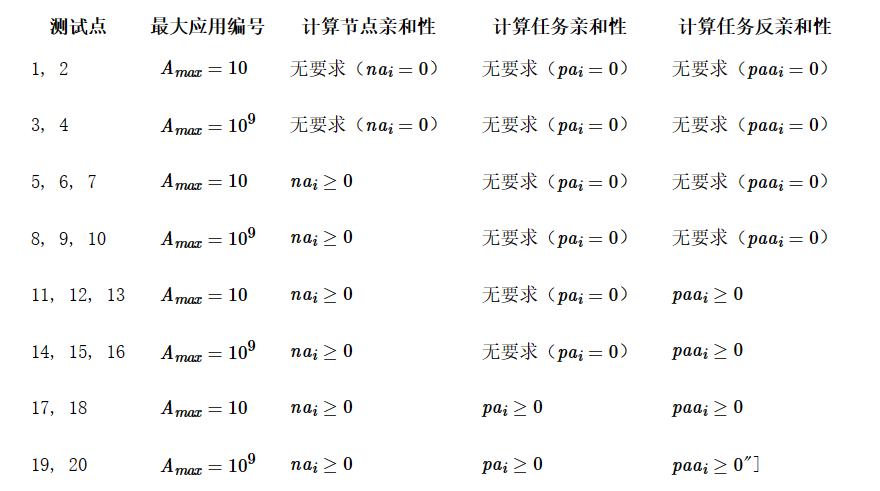
\includegraphics[width = 5in]{测试数据.png}
    \caption{测试数据}
\end{figure}
\newpage
\subsection{题解}
\subsubsection{解法一 (100分)}
\par 定义结构体 $Node$ 存放每个计算节点的编号,所在可用区,运行计算任务的数量,同时定义$set$ <$int$> $task$ 存放当前节点运行的计算任务的编号。定义 $vector$<$int$> $node$存放 $Node$。在筛选过程中,定义 $vector$<$int$> $temp$ 用于筛选计算节点。筛选完后根据题意使用 $std::sort$ 对剩余节点进行排序,取首元素并对相应 $Node$ 的状态进行更新。
\par 具体筛选方法如下:
\begin{itemize}
    \item 计算节点亲和性:遍历 $temp$,若 $node[i].block != na$,则删除该计算节点。
    \item 计算任务亲和性:定义 $set$<$int$> $temp\_s$,首先遍历 $node$ 数组,若 $node[i].task$ 中存放有对应计算任务,则将其 $block$ 插入 $temp\_s$ 中,接下来遍历 $temp$ 数组,若 $node[i].block$ 在 $temp\_s$ 中未出现,则删除该计算节点。
    \item 计算任务反亲和性:定义数组 $temp2$, 将经过上述程序筛选后的 $temp$ 赋值给 $temp2$。遍历 $temp2$,若 $node[i].task$ 中存放有对应计算任务,则删除该计算节点。
    \item 对于筛选完的 $temp、temp2$,若 $temp2$ 为空并且 $paar=1$,或 $temp$ 为空,则该计算任务无法分配。
\end{itemize}
\par 需要注意的是,如果直接定义 $cmp$ 函数使用 $std::sort$ 进行自定义排序会 $TLE$,只能通过 $80\%$的数据。因此这里采用 $lambda$ 表达式实现,可通过 $100\%$的数据。
\begin{itemize}
    \item 时间复杂度:$O(n^2logn)$
\end{itemize}
\subsubsection{C++ 代码实现}
\lstinputlisting[
    style = C++,
    title = {\bf 202203-3 计算资源调度器}
]{test03.cpp}


\section{202203-4 通信系统管理}
\begin{itemize}
    \item 时间限制:$2.0\texttt{ s}$
    \item 空间限制:$512.0\texttt{ MB}$
\end{itemize}
\subsection{题目}
\subsubsection{问题描述}
\par 有 $n$ 台计算机,互相之间可以发送数据。任意两台机器之间每日可以互相发送的数据量有限(每日可用额度),并且有如下定义:
\begin{itemize}
    \item 主要通信对象:每台机器的 通信主要对象 为当前时刻与该机器的每日可用额度最大的机器(并列取编号最小)。若其为 $0$,则该机器无 主要通信对象 。
    \item 通信孤岛:若一台机器与任何机器之间的每日可用额度均为 $0$,则称为 通信孤岛 ,并认为其无 主要通信对象 。
    \item 通信对:若两台机器之间互为主要通信对象,则称为 通信对 。
\end{itemize}
\par 在 $1 \sim m$ 时间内,每天都要处理若干额度申请,每个申请如 $u$ $v$ $x$ $y$ 格式,表示机器 $u$ $v$ 之间每日可用额度增大 $x$,持续 $y$ 天;而后,需要查询若干机器的主要通讯对象;最后,可能需要查询此时刻的通信孤岛和通信对个数。
\subsubsection{子任务}
\par 设 $A=\sum_{i = 1}^{m}k_i$,$B=\sum_{i = 1}^{m}l_i$。
\par 子任务 $1$ (20分):满足 $n,m \leq 1000$, $A,B \leq 2000$;
\par 子任务 $2$ (10分):满足 $p_i = q_i = 0$;
\par 子任务 $3$ (10分):满足 $l_i = q_i = 0$;
\par 子任务 $4$ (15分):满足 $l_i = 0$;
\par 子任务 $5$ (10分):满足 $k_1 = A$,对于所有额度申请均满足 $y = m$;
\par 子任务 $6$ (15分):满足 对于所有额度申请均满足 $y = m$;
\par 子任务 $7$ (20分): 无特殊性质;
\par 对于 $100\%$ 的数据,$1 \leq n,m \leq 10^5$,$1 \leq A,B \leq 2\times 10^5$,$1 \leq u,v \leq n$,$1 \leq x \leq 10^9$,$1 \leq y \leq m$。
\par 所有额度申请均满足 $u \neq v$。
\subsection{题解}
\subsubsection{解法一 (100分)}
\par 考虑使用邻接表存储信息。同时,因为题目需要查询某个机器的通信主要对象,可以定义结构体 $Node$,并重载 $<$ 运算符,使用 $set$ 容器维护 $Node$。同时,用 $map$ 映射机器 $u$ $v$ 之间的可用额度。在每一时刻更新节点状态和孤岛、通信对数量,按题目要求模拟即可。
\par PS:由于本题数据规模大,务必使用快读读入数据,否则会 $TLE$。
\begin{itemize}
    \item 时间复杂度:$O(m(Tlogn))$
\end{itemize}
\subsubsection{C++ 代码实现}
\lstinputlisting[
    style = C++,
    title = {\bf 202203-4 通讯系统管理}
]{test04.cpp}


\section{202203-5 博弈论与石子合并}
\begin{itemize}
    \item 时间限制:$1.0\texttt{ s}$
    \item 空间限制:$512.0\texttt{ MB}$
\end{itemize}
\subsection{题目}
\subsubsection{问题描述}
\par 小 $z$ 和小 $c$ 准备玩 $Nim$ 游戏,他们准备了一共 $n$ 堆石子,从左到右第 $i$ 堆石子的数量为 $a_i$。游戏规则如下:
\par 两人轮流操作,每次操作可以选择将两堆相邻的石子合并,或扔掉最左边或最右边的石子,且不能不操作,直至只剩下一堆石子。
\par 现假设小 $z$ 希望最后剩下的石子尽量多,小 $c$ 希望尽量少,且二人的大脑与量子计算机平分秋色,问最后这堆石子的数量。
\subsubsection{子任务}
\par 子任务 $1$ (20分):$n \leq 20$,无特殊性质;
\par 子任务 $2$ (20分):$n \leq 10^5$,每堆石子大小相等;
\par 子任务 $3$ (20分):$n \leq 10^5$,$n$ 是偶数,且小 $z$ 先手;
\par 子任务 $4$ (20分):$n \leq 10^5$,$n$ 是偶数,且小 $c$ 先手;
\par 子任务 $5$ (5分):$n \leq 2000$,无特殊性质;
\par 子任务 $6$ (15分):$n \leq 10^5$,无特殊性质;
\par 对于 $100\%$ 的数据,$1 \leq n \leq 10^5$,$0 \leq k \leq 1$,$a_i > 0$,$\sum_{i = 1}^{n}a_n \leq 10^9$。
\subsection{题解}
\subsubsection{解法一 (100分)}
\par 根据题意,我们可以将问题分解为两部分:
\begin{itemize}
    \item 小 $z$ 操作时剩余堆数为偶数:从小 $c$ 的角度看,如果小 $z$ 选择合并的不是中间的两堆石子,则无论之后小 $z$ 如何操作,该堆石子都会被小 $c$ 扔掉,所以小 $z$ 只能合并中间两堆石子,这种情况下小 $c$ 束手无策,只能气急败坏地尽可能多丢掉一些石子。由于小 $c$ 只能操作 $\frac{n}{2} - 1$ 次。所以问题转化为求 $\sum_{i = j}^{j + \frac{n}{2}}a_i$ $(1 \leq j \leq \frac{n}{2})$ 的最小值。
    \item 小 $z$ 操作时剩余堆数为奇数:设 $sum_i = \sum_{i = j}^{k}a_i$ $(1 \leq j \leq k \leq n)$,由上论述可知,此情况下无论小 $z$ 选择合并哪两堆,小 $c$ 都可以将其扔掉。而小 $c$ 只能操作 $\frac{n}{2}$ 次,也就是只能扔掉 $\frac{n}{2}$ 堆石子。因此,小 $z$ 只能广布局,将某些堆合并,同时,为了保证合并后的堆不全被小 $c$ 扔掉,合并后的堆的数量应大于 $\frac{n}{2}$,且最后剩下的一定是数量最小的一堆。 所以,问题转化成寻求一个尽可能大的 $x$,使$sum_i \geq x$,同时这样的堆数应大于 $\frac{n}{2}$。
\end{itemize}
\par PS:对于情况二,我们很容易得出 $x$ 即为最后的答案:
\begin{itemize}
    \item 若 $\exists sum_i = x$,由于小 $c$ 希望尽可能小,所以会将大于 $x$ 的堆扔掉。
    \item 若 $\forall sum_i > x$,说明 $x+1$ 对于情况二也成立,此时 $x$ 并非最终解。
\end{itemize}
\begin{itemize}
    \item 时间复杂度:$O(nlogn)$
    \item 空间复杂度:$O(2n)$
\end{itemize}
\subsubsection{C++ 代码实现}
\lstinputlisting[
    style = C++,
    title = {202203-5 博弈论与石子合并}
]{test05.cpp}
\end{document}
